\documentclass{article}

\usepackage{tikz} 
\usetikzlibrary{automata, positioning, arrows} 

\usepackage{amsthm}
\usepackage{amsfonts}
\usepackage{amsmath}
\usepackage{amssymb}
\usepackage{fullpage}
\usepackage{color}
\usepackage{parskip}
\usepackage{float}
\usepackage{hyperref}
  \hypersetup{
    colorlinks = true,
    urlcolor = blue,       % color of external links using \href
    linkcolor= blue,       % color of internal links 
    citecolor= blue,       % color of links to bibliography
    filecolor= blue,        % color of file links
    }
    
\usepackage{graphicx}
    
\usepackage{listings}
\usepackage[utf8]{inputenc}                                                    
\usepackage[T1]{fontenc}                                                       

\definecolor{dkgreen}{rgb}{0,0.6,0}
\definecolor{gray}{rgb}{0.5,0.5,0.5}
\definecolor{mauve}{rgb}{0.58,0,0.82}

\lstset{frame=tb,
  language=haskell,
  aboveskip=3mm,
  belowskip=3mm,
  showstringspaces=false,
  columns=flexible,
  basicstyle={\small\ttfamily},
  numbers=none,
  numberstyle=\tiny\color{gray},
  keywordstyle=\color{blue},
  commentstyle=\color{dkgreen},
  stringstyle=\color{mauve},
  breaklines=true,
  breakatwhitespace=true,
  tabsize=3
}

\newtheoremstyle{theorem}
  {\topsep}   % ABOVESPACE
  {\topsep}   % BELOWSPACE
  {\itshape\/}  % BODYFONT
  {0pt}       % INDENT (empty value is the same as 0pt)
  {\bfseries} % HEADFONT
  {.}         % HEADPUNCT
  {5pt plus 1pt minus 1pt} % HEADSPACE
  {}          % CUSTOM-HEAD-SPEC
\theoremstyle{theorem} 
   \newtheorem{theorem}{Theorem}[section]
   \newtheorem{corollary}[theorem]{Corollary}
   \newtheorem{lemma}[theorem]{Lemma}
   \newtheorem{proposition}[theorem]{Proposition}
\theoremstyle{definition}
   \newtheorem{definition}[theorem]{Definition}
   \newtheorem{example}[theorem]{Example}
\theoremstyle{remark}    
  \newtheorem{remark}[theorem]{Remark}

\title{CPSC-406 Report}
\author{Your Name  \\ Chapman University}

\date{\today} 

\begin{document}

\maketitle

\begin{abstract}
\end{abstract}

\setcounter{tocdepth}{3}
\tableofcontents

\section{Introduction}\label{intro}

\section{Week by Week}\label{homework}

\subsection{Week 1}

\subsubsection{Exercise 1: Word Processing with DFAs}

\textbf{Notes and Homework:}

\begin{figure}[H]
  \centering
  \includegraphics[width=0.8\textwidth]{../BkD7CQiYJe.jpg}
  \caption{Automata $A_1$ and $A_2$}
\end{figure}

\begin{figure}[H]
  \centering
  \includegraphics[width=0.8\textwidth]{../Bk0mRmjYJg.jpg}
  \caption{Additional automata reference}
\end{figure}

\textbf{Question 1:} Which of the following words are accepted/refused by $A_1$ and $A_2$, respectively? Complete the table.

\begin{table}[H]
  \centering
  \renewcommand{\arraystretch}{1.2}
  \begin{tabular}{|c|c|c|}
    \hline
    $w$ & accepted by $A_1$? & accepted by $A_2$? \\ \hline
    $aaa$ & no & yes \\ \hline
    $aab$ & yes & no \\ \hline
    $aba$ & no & no \\ \hline
    $abb$ & no & no \\ \hline
    $baa$ & no & yes \\ \hline
    $bab$ & no & no \\ \hline
    $bba$ & no & no \\ \hline
    $bbb$ & no & no \\ \hline
  \end{tabular}
  \caption{Acceptance table for $A_1$ and $A_2$}
\end{table}

\textbf{Question 2:} More generally, can you completely describe the languages $L(A_k)$ accepted by $A_k$, for $k = 1, 2$?

The language $L(A)$ accepted by this DFA is:
$$L(A) = \{ w \in \{a,b\}^* \mid \text{the number of } a \text{'s in } w \text{ is even} \}$$

\subsubsection{Exercise 2: Designing DFAs}

Design DFAs whose accepted languages are given as follows:

\begin{enumerate}
  \item All the words that end with $ab$
  \item All the words that contain $ab$
  \item All the words that contain an odd number of $a$'s and an odd number of $b$'s
  \item All the words that contain an even number of $a$'s and an odd number of $b$'s
  \item All the words such that any three consecutive characters contain at least one $a$
  \item All the words that contain $aba$
\end{enumerate}

\textbf{DFA Diagrams:}

\begin{figure}[H]
  \centering
  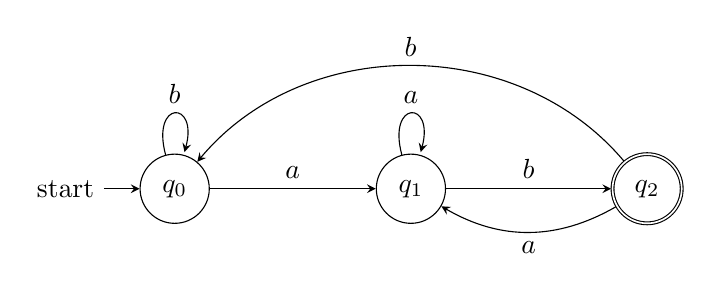
\begin{tikzpicture}[node distance=3cm, ->, >=stealth]
    \node[state, initial] (q0) {$q_0$};
    \node[state] (q1) [right of=q0] {$q_1$};
    \node[state, accepting] (q2) [right of=q1] {$q_2$};
    
    \path (q0) edge [loop above] node {$b$} (q0);
    \path (q0) edge [above] node {$a$} (q1);
    
    \path (q1) edge [loop above] node {$a$} (q1);
    \path (q1) edge [above] node {$b$} (q2);
    
    \path (q2) edge [bend left=30, below] node {$a$} (q1);
    \path (q2) edge [bend right=50, above] node {$b$} (q0);
  \end{tikzpicture}
  \caption{DFA for words ending with $ab$}
\end{figure}

\vspace{0.3cm}

\textbf{Observation:} Compare the various automata designed above. What patterns do you notice in their structure and complexity?

\section{Synthesis}

\section{Evidence of Participation}

\section{Conclusion}\label{conclusion}

\begin{thebibliography}{99}
\bibitem[BLA]{bla} Author, \href{https://en.wikipedia.org/wiki/LaTeX}{Title}, Publisher, Year.
\end{thebibliography}

\end{document}